\subsection{Decision Tree} \label{subsec: decisiontree}
Decision trees are a good manner to figure out, which parts of the data set have the most influence on the decision. We used again \textbf{RapidMiner} for building trees based on different data sets. 

\begin{figure}[!htbp]
\centering
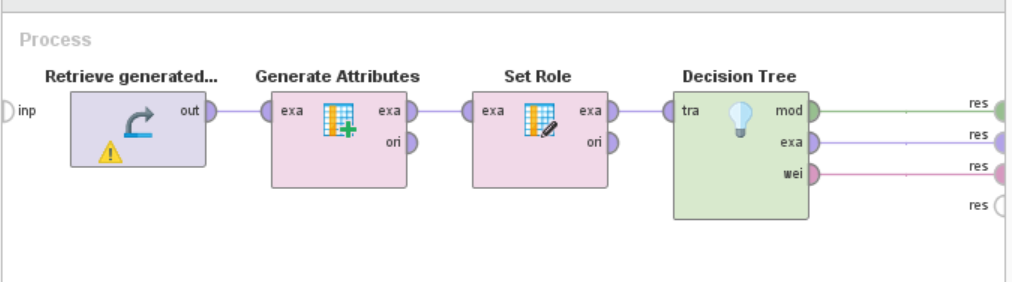
\includegraphics[width = 0.9\textwidth]{DecisionTreeRapidModel.PNG}
\caption{Process for decision trees in RapidMiner}
\label{fig: RapDec}
\end{figure}

RapidMiner does the following steps, to see in figure \ref{fig: RapDec}:
\begin{description}
	\item[Retrieve] includes the dataset
	\item[Generate Attribute] changes the Numerical Attribute strata to four binomial ones
	\item[Set Role] gives strata the label role, so that the decision tree has those as leafs
	\item[Decision Tree] creates the decision tree
\end{description}

Furthermore we choose information gain as splitting criterium (minimal gain 0.1) and a confidence of 0.25. Other configuration does not show different results.

In the first step we applied the process on the whole data set and the resulting tree was just the leaf "strata 2". So we tried it with different other data sets and the best result we got was for \textbf{stratified person data} equally distributed 3 stratas and just 200 in every aggerated strata group.

\begin{figure}[!htbp]
\centering
\begin{subfigure}{0.7\textwidth}
\includegraphics
{}